\documentclass{article}

\usepackage{xcolor}
\usepackage{graphicx}
\usepackage{float}
\usepackage{verbatim}
\usepackage{amssymb}
\usepackage{amsmath}
\usepackage{hyperref}
\usepackage{authblk}
\usepackage{algpseudocode}
\usepackage{algorithm}

\setlength\itemsep{1em}
\hyphenation{E-the-re-um at-tes-ta-tion}

\title{Effective Quality of Lighthouse's\\Greedy Approach to Attestation Packing}
\author{Satalia \& Sigma Prime}

\begin{document}

\maketitle{}

\begin{abstract}
We experimentally assess the quality of the approach for solving the
Attestation Aggregation and Packing Problem (AAPP, \cite{Satalia22a})
implemented in Sigma Prime's Lighthouse client. Lighthouse's approach is
composed of two greedy stages (aggregation and packing) executed in sequence.
The latter is based on an approximation algorithm for the weighted maximum
coverage problem, and is guaranteed to find solutions non-worse than $1-1/e
\approx 0.632$ of the optimum. However, while the theoretical results provide a
lower bound on the packing quality, they give no indication of the algorithm's
behavior when applied to typical instances of the AAPP. Moreover, there is no
theoretical result on the performance of the first stage (aggregation).

In order to shed some light on the algorithm's expected behavior in the
typical case, we take advantage of the exact MIP approach outlined in
\cite{Satalia22b} and carry out an experimental analysis on eight days-worth of
instances extracted by Sigma Prime from Ethereum's Beacon chain. The MIP
approach is guaranteed to find the optimal aggregation and packing, and we can
therefore benchmark Lighthouse's approach against it.
\end{abstract}

\tableofcontents


\section{Introduction}

In this report we outline the experimental analysis that we carried out to
assess the typical quality obtained by Lighthouse's greedy approach for solving
the AAPP. The cornerstone of this analysis is the exact approach described in
\cite{Satalia22b} to find optimal solutions to the AAPP, which the greedy
approach can be benchmarked against.

The report is organized as follows. Section \ref{sec:setup} outlines the
experimental setup. Section \ref{sec:results} provides a summary of the raw
results, in particular with respect to the key aspects of interest: quality and
run time, and some discussion of them. Finally, Section \ref{sec:next} outlines
some possible directions for this work, to be picked up in Phase 2.

\section{Experimental setup} \label{sec:setup}

This section aims at providing a detailed description of how the experiments
were carried out. We will cover both the instances and the approach.

\subsection{Instances}

We have used $\approx 8$ days worth of instances, each one corresponding to one slot (i.e., one
block proposal) of Ethereum's Beacon chain. Table~\ref{tab:insta} illustrates
some of the variability that can be observed throughout the instances. We
see that most instances have a number of attesters around the $12000$ mark,
and a number of unique attestation data in the $\left[200,400\right]$ range.

\begin{table}[h!]
  \centering
    \begin{tabular}{lrrrrr}
    \hline
    \textbf{Percentiles}    & \multicolumn{1}{c}{\textbf{0\%}} & \multicolumn{1}{c}{\textbf{25\%}} & \multicolumn{1}{c}{\textbf{50\%}} & \multicolumn{1}{c}{\textbf{75\%}} & \multicolumn{1}{c}{\textbf{100\%}} \\ \hline
    Attesters               & 3461                             & 11729                             & 11859                             & 12077                             & 73999                              \\
    Unique attestation data & 83                               & 205                               & 277                               & 372                               & 1441                               \\ \hline
    \end{tabular}
  \caption{Basic statistics on the instances used in this analysis.\label{tab:insta}}
\end{table}

Each instance comes with the corresponding greedy solution as computed by
Lighthouse, however the total reward was recalculated by us.  The instances
have been provided in the JSON format described in \cite{Satalia22a}.

\paragraph{Note.} The instances reflect the relatively quiet state of the
Beacon blockchain, which is not used for real transactions at the time of this
writing. One could expect numbers to increase as the chain gains more adoption.

\subsection{Approach}

We have identified an optimum for each instance by using the MIP approach
described in \cite{Satalia22b}. Although the approach is discussed at length
in a separate report, here are the main steps.

\begin{enumerate}
  \item \textbf{Compute the set of candidate attestations.} This is the union
  of the candidate attestations for each unique attestation data. These are
  obtained as follows
    \begin{enumerate}
      \item enumerate all the attestations corresponding to maximal cliques for
      the graph where the vertices represent aggregated attestations, and the
      edges encode the disjointness of their attester sets (this is carried
      out using the variant of the Bron-Kerbosch approach described in 
      \cite{Satalia22b}) with the various mentioned optimisations,
      \item extend the above with all the compatible unaggregated attestations,
      \item add to the above a further aggregated attestation made up of all
      unaggregated attestations.
    \end{enumerate}
  \item \textbf{Solve a maximum weighted coverage problem.} This is a problem
  with maximum capacity 128, and where each set corresponds to one of the above
  candidate attestations, and each element corresponds to an attester with a
  weight identical to its inclusion reward. We solve this problem using the MIP
  model outlined in \cite{Satalia22b}.
\end{enumerate}

\noindent
All of the code to carry out the above steps is developed in Rust, to keep
consistency with the Lighthouse codebase, and to facilitate any further
development to be carried out in Phase 2.  While performance wasn't a key issue
for Phase 1 (beyond the practical implication of running the approach for a
large number of instances), we have taken steps to avoid any unnecessary
computation.

We have used the \texttt{good\_lp}\footnote{See
\href{https://crates.io/crates/good_lp}{good\_lp}.} crate for modeling and
solving the weighted maximum coverage MIP model. \texttt{good\_lp} provides a
convenient modeling layer and bindings for many available MIP solvers (more on
this later), and for these experiments we used the CBC solver \cite{Forrest05}
due to its widespread availability.

\section{Results} \label{sec:results}

With this experiment, we wanted to answer two main questions:
\begin{itemize}
  \item How large is the gap between greedy and optimal solutions?
  \item How well does the MIP solver perform, compared to production
    requirements?
\end{itemize}

\subsection{Optimality gap}

Experimental results show that it exists, but, outside of certain outliers,
the relative gap is very small. To illustrate the distribution of the relative
gap, we provide a table of relative gap thresholds and how often they're
exceeded.

\begin{center}
\begin{tabular}{ |c|c| }
  \hline
  Threshold & \% of instances where gap $>$ threshold \\
  \hline
  0\% & 47.68\% \\
  1\% & 0.14\% \\
  5\% & 0.03\% \\
  \hline
\end{tabular}
\end{center}

This shows that roughly 52\% of the time the greedy solution was already
optimal, and that in only 14 of the 51 097 instances was the gap greater
than 5\%.

Ultimately, the average relative gap was 0.2\%, or, in absolute terms,
261 836 297 Gwei over the data collection period.

\subsection{Solver performance}

While the current solver isn't fit for production, its performance time-wise
can still be considered an upper bound for other optimal solutions. Results
show that even optimal solutions should be able to perform at production speeds without
too much trouble.
%
\begin{figure}[!ht]
  \centering
  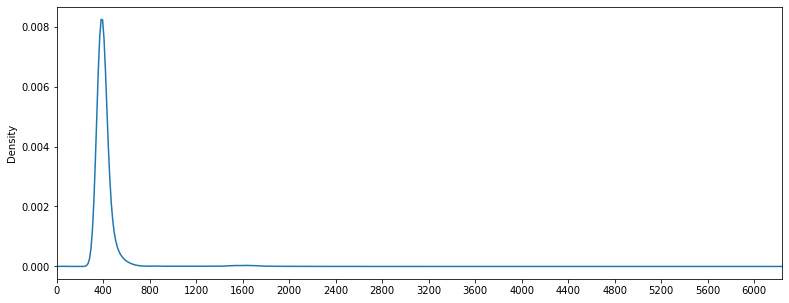
\includegraphics[width=1\textwidth]{mip_density.png}
  \caption{A density plot of solver run times.\label{fig:mip_density}}
\end{figure}
%

And, to illustrate the outlier run times, a table of run time thresholds and
how often they're exceeded.

\begin{center}
\begin{tabular}{ |c|c| }
  \hline
  Threshold & \% of instances where run time $>$ threshold \\
  \hline
  1000 ms & 1.41\% \\
  2000 ms & 0.14\% \\
  3000 ms & 0.04\% \\
  4000 ms & 0.03\% \\
  5000 ms & 0.02\% \\
  6000 ms & 0.00\% \\
  \hline
\end{tabular}
\end{center}

While performance is good most of the time, it can slow down to unacceptable
speeds every once in a while. This leads us to believe that it's possible to
find an optimality-reaching solution that achieves good performance.

The answers to both of our questions should be caveated with the fact that this
is based on current data, on current chain activity. As time goes on, the
activity on the chain, and thus these results, could change. However, these
results still let us make a few observations.

\subsection{Aggregating is fast, packing is slow}

The approach we use for identifying the candidate attestations to include in a
block is very fast (usually $\approx 15ms$ or around $3-4\%$ of the total run
time). The rest ($\approx 96-97\%$) of the time is spent solving the MIP model
for the weighted maximum coverage problem. This figure is at least partially
explained by the choice of the MIP solver. For reference, the average run time
of CBC on a standard set of MIP problems is more than 8 times larger than
Gurobi's \cite{gurobi} (the leading commercial MIP solver). Having said that,
using a commercial solver will require users to own a license, and that may
not be desirable.  

On the other hand, the fact that optimality-preserving candidate attestations
can be computed efficiently suggests a possible improvement of Lighthouse's
current heuristic, which is online and greedy and has no theoretical
guarantees.

\subsection{Lighthouse's approach: practice vs. theory}

From the results presented in the previous section, it is clear that the greedy
approach finds the optimum quite often (at least on this particular data set)
and, when it doesn't, it doesn't typically get very far from it.  There are a
few pathological cases where the gap is much larger (e.g., $\approx 40\%$ off
the optimum) but these are not common, and at this stage we cannot assess if it
is due to Lighthouse's greedy aggregation stage, or its greedy packing stage. 

At any rate, when factoring in both solution quality and run time, the approach
seems to strike a reasonable balance that yields profitable proposals most of
the time.

Qualifying the (financial) loss in profit for the cases where Lighthouse's
approach doesn't reach the optimum is beyond the scope of this experimental
evaluation. However, from an optimisation perspective, it may make sense to
investigate methods that are either exact and sufficiently fast or that, while
not being exact, can deliver better performance than the current approach more
frequently.

\subsection{Performance of the MIP solver}

While we were not aiming for real-time performance for Phase 1 of this project,
we were positively surprised by the performance of the MIP approach, which
allowed to find optimal solutions for the packing part of the problem in less
than $0.5s$ more than $93\%$ of the time. 

We have some intuition around this. Here are what we think may be the main
contributors.

\begin{itemize}
  \item \textbf{Scale}. The number of \emph{decision variables} (i.e., the ones
  modeling whether a given attestation is added to the block or not) is rather
  low, often within a few thousands. This is only possible because the job of
  restricting the search space to the cliques that are maximal with respect to
  attester coverage has been dealt with at the previous step.  \item
  \textbf{Additive contribution}. Each distinct attestation data comes with a
  handful of aggregated attestations which overlap in terms of attester
  coverage, i.e., including one of them in the solution affects the
  contribution of including the others. This is not the case for attestations
  with different attestation data, which are the majority. For these, the
  contribution is additive, and choosing one doesn't affect the value of
  choosing another. Depending on its implementation, a solver may be able to
  use this information to obtain efficient bounds on the maximum reward that
  can be achieved when extending a solution with an attestation. Calculating
  tight bounds is one of the key strategies MIP solvers use to avoid searching
  non-promising parts of the search space.
\end{itemize}

\noindent
Even if the performance of the MIP approach is better than we expected, there
are two main challenges to its inclusion in Lighthouse. 

\begin{enumerate}
  \item The performance may not be enough for the real-time scenario, where
  it matters how quickly a validator can propose a new block. In particular,
  the run time of the MIP approach varies quite wildly from $\approx 200ms$
  to more than $6s$.
  \item The MIP solver would represent a dependency, which would have to be
  audited properly in order to be trusted\footnote{Note that, while the first
  point could be mitigated with the decomposition method that we proposed in
  \cite{Satalia22b}, if said method relies on the MIP approach, a MIP solver
  would still be a dependency.}, in this sense it may be better to use an
  approach that can be fully included in Lighthouse's codebase and audited
  accordingly.
\end{enumerate}

\noindent
In Section \ref{sec:next} we discuss some possible alternatives to the MIP
approach.

\subsection{Predicting metrics of interest}

We have tracked some of the performance indicators of interest, namely
%
\begin{itemize}
  \item time taken by the MIP to find an optimal solution,
  \item optimality gap of the greedy solution, i.e., the relative
  difference in quality between the quality of the greedy solution
  and the quality of the optimal solution,
\end{itemize}
%
and explored their relationship with measurable features (both of the instance
and of the output of the aggregation phase). 

\paragraph{MIP run time.} It appears that there is a relatively strong linear
correlation between the number of attesters, the number of unique attestation
data, and the performance of the MIP solver. A simple linear model can predict
the time taken by the MIP solver to find a solution with a reasonable accuracy
($R^{2} \approx 0.84$). Let $a$ be the number of attesters in the instance, and
$d$ the number of unique attestation data, then the expected time (in
milliseconds) $p$ to solve the MIP model is

\begin{equation}
  p = -597.85 + a \times 0.085 + d \times -0.093.
\end{equation}

\noindent
This is something that can be used to estimate, for instance, how this
particular MIP approach would scale as the size of the instances change. We
imagine that both $a$ and $d$ would increase as the Beacon blockchain is
adopted, which would drive up the expected run time of the MIP approach.

\paragraph{Optimality gap.} Unfortunately, we haven't found any clear
correlation between measurable features and the optimality gap. It would be
interesting to understand what makes a problem hard to solve for the greedy
approach, but at this stage there isn't a clear feature explaining this metric.

\section{Future work} \label{sec:next}

We have outlined a few areas for future research, these are areas that we are
confident could achieve the goal of Phase 2, i.e., building an approach that
can be used in production and performs better than the current. Broadly
speaking, these revolve around exploring approaches inbetween the exact MIP
approach and the greedy approach implemented by Lighthouse (see
blue area in Figure~\ref{fig:future}).
%
\begin{figure}[!ht]
  \centering
  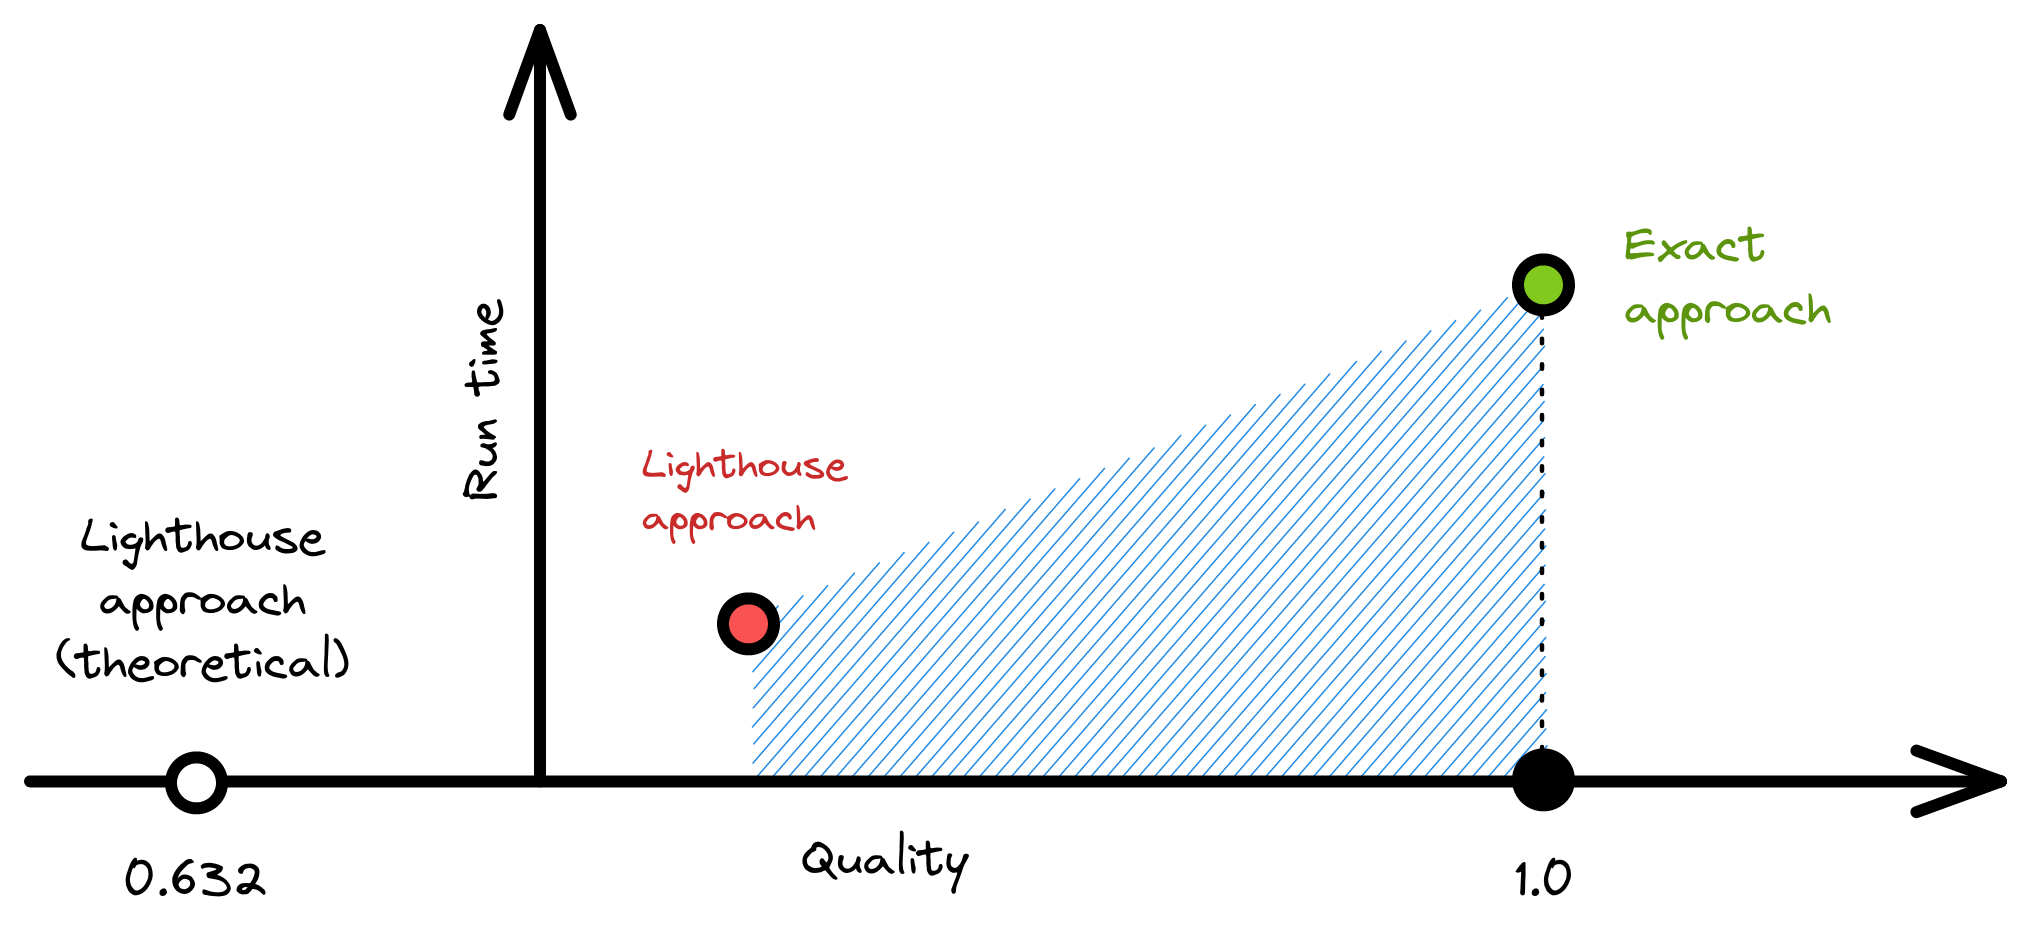
\includegraphics[width=.8\textwidth]{future.png}
  \caption{Spaces of approaches to be explored.\label{fig:future}}
\end{figure}
%
The rest of this section will outline some more specific directions.

\subsection{Decomposition approach}

Due to the fact that the MIP approach was sufficient to fulfil the scope of
Phase 1, we haven't needed to implement the decomposition approach outlined in
\cite{Satalia22b}. It is our belief that the decomposition approach
would perform significantly better than the MIP approach. Our belief is based
on the following observations
\begin{enumerate}
  \item solving the weighted maximum coverage problem represents the highest
  time spender in the MIP approach,
  \item the weighted maximum coverage problem is NP-hard, therefore solving
  large problem is much harder than solving small problems, and
  \item the decomposition approach involves solving much smaller weighted
  maximum coverage problems.
\end{enumerate}
We therefore believe that this is a meaningful line of research.

\subsection{Replacing the MIP approach}

So far we have solved the weighted maximum coverage problem using a MIP
solver. Because of the limitations outlined previously around using a MIP
within Lighthouse, we have considered other options to replace the MIP. 

The one that currently seems most promising, but only applicable in the context
of a decomposition approach, is a branch \& bound approach based on a
backtracking search. There are several bounds that we can use to speed-up this
type of search, and the added complexity to the Lighthouse codebase would be
limited. Moreover, it wouldn't require any additional library, removing the
uncomfortable dependency on third-party IP. 

\subsection{Pruning candidate attestations}

There are some strategies that can be used to further reduce the size of the
weighted maximum coverage problems to be solved, e.g., pruning attestations
that are dominated by others with respect to attester coverage. These
strategies require additional computations, and we cannot exclude that the
additional computation could outweight the advantage of dealing with a smaller
problem, therefore an appropriate trade-off between pre-processing and solving
must be identified (possibly experimentally).

\subsection{Other heuristic approaches}

Exact approaches are not the only possibility when it comes to Phase 2.
Depending on the \emph{definition of good}, we may want to consider heuristics
that don't guarantee optimality, but that perform better than the current
approach. These could even combine some of the components already developed
for Phase 1 with new logic. Some examples are

\begin{enumerate}
  \item greedy approach $\rightarrow$ local search,
  \item maximal clique enumeration $\rightarrow$ greedy approach,
  \item maximal clique enumeration $\rightarrow$ greedy approach $\rightarrow$
  local search,
  \item maximal clique enumeration $\rightarrow$ branch \& bound.
\end{enumerate}

\noindent
These would be compared experimentally, and the corresponding quality
\emph{vs.} complexity trade-off would be evaluated.

\section*{Acknowledgments}

We thank Sigma Prime for their support in providing the details of the AAPP, as
well as a sample of instances from Ethereum's Beacon chain. 

\bibliographystyle{plain}
\bibliography{report}

\end{document}
